\documentclass[11pt,a4paper]{article}
\usepackage[margin=1in]{geometry}
\usepackage[T1]{fontenc}
\usepackage[utf8]{inputenc}
\usepackage{lmodern}
\usepackage{microtype}
\usepackage{amsmath,amssymb,amsthm}
\usepackage{booktabs}
\usepackage{graphicx}
\usepackage{xcolor}
\usepackage{siunitx}
\usepackage{hyperref}
\usepackage{enumitem}
\usepackage{fancyhdr}
\usepackage{titlesec}
\usepackage{setspace}
\usepackage{caption}
\usepackage{subcaption}
\usepackage{float}

\hypersetup{
  colorlinks=true,
  linkcolor=blue!60!black,
  citecolor=blue!60!black,
  urlcolor=blue!60!black
}

\pagestyle{fancy}
\fancyhf{}
\lhead{QSH Research Report}
\rhead{\thepage}

\titleformat{\section}{\large\bfseries}{\thesection.}{0.5em}{}
\titleformat{\subsection}{\normalsize\bfseries}{\thesubsection.}{0.5em}{}

\title{\textbf{QSH: A Quantum-Inspired Secure Shell Protocol}\\
\large Simulated BB84 Key Exchange, Authenticated Encryption, and Remote Session Services}
\author{Research Prototype Report}
\date{\today}

\begin{document}
\maketitle
\begin{abstract}
This report presents QSH, a research protocol inspired by SSH that combines a simulated BB84 quantum key distribution (QKD) stage with a classical encrypted communication layer. The implementation uses Qiskit/AerSimulator for qubit-level BB84 simulation, HKDF-SHA256 for key derivation, AES-GCM for authenticated transport, and an encrypted post-handshake password-authentication phase. QSH supports persistent remote shell sessions and secure file transfer over a single established channel. We also model an active eavesdropper (Eve) through intercept-resend strategies, including both random-basis and biased-basis attacks, and quantify protocol behavior through Monte Carlo experiments. The generated results demonstrate a clear relationship between interception rate and observed QBER, supporting the core BB84 intuition that stronger interception increases detectability and reduces handshake acceptance probability. We discuss security properties, limitations of simulation-based quantum modeling, and practical implications for protocol experimentation.
\end{abstract}

\tableofcontents
\newpage

\section{Introduction}
Secure remote administration protocols, most notably SSH, rely on strong classical cryptography for confidentiality, integrity, and endpoint authentication. QSH explores a different educational direction: integrating a \emph{quantum-inspired} key establishment stage using a simulated BB84 protocol, then switching to standard authenticated encryption for application traffic.

The objective is not to replace production SSH, but to create an experimentally meaningful framework for investigating:
\begin{itemize}[leftmargin=1.5em]
  \item how BB84-like key establishment behaves under noise and adversarial interception,
  \item how a sifted QKD key can feed a classical key schedule (HKDF),
  \item how protocol-level services (shell, file transfer, persistent sessions) can be layered on top of a secure channel.
\end{itemize}

QSH is implemented in Python, with:
\begin{itemize}[leftmargin=1.5em]
  \item \texttt{qiskit} + \texttt{qiskit-aer} for single-qubit state preparation and measurement simulation,
  \item \texttt{cryptography} for HKDF and AES-GCM,
  \item JSON-framed message transport over TCP sockets.
\end{itemize}

This report documents protocol design, implementation mapping, empirical evaluation, and adversarial analysis.

\section{Background and Motivation}
\subsection{BB84 Intuition}
In BB84, Alice encodes random bits in random bases (computational $Z$ or Hadamard $X$). Bob measures each qubit in a random basis. After basis disclosure, only matching-basis outcomes are retained (sifting). A public sample is compared to estimate the quantum bit error rate (QBER). Excessive QBER suggests channel noise or eavesdropping.

Eve's intercept-resend attack perturbs the channel: when Eve chooses the wrong measurement basis, she probabilistically disturbs the transmitted state, causing elevated QBER at Bob.

\subsection{Why a Hybrid Protocol}
QKD alone does not provide a full remote management stack. QSH therefore uses BB84 output as \emph{entropy input} into a classical cryptographic channel:
\begin{enumerate}[leftmargin=1.5em]
  \item BB84 simulation and sifted-bit extraction,
  \item HKDF-based session-key derivation,
  \item AES-GCM protected transport for command and file operations.
\end{enumerate}

This separation provides architectural clarity and allows controlled experiments on the QKD stage while preserving practical message confidentiality/integrity in transport.

\section{Quantum-Theoretic Foundations}
\subsection{Postulates and State Representation}
QSH's BB84 stage is grounded in standard quantum-information postulates. A qubit lives in a two-dimensional Hilbert space:
\[
\lvert \psi \rangle = \alpha \lvert 0 \rangle + \beta \lvert 1 \rangle,\quad \alpha,\beta \in \mathbb{C},\quad |\alpha|^2 + |\beta|^2 = 1.
\]
Measurement probabilities follow Born's rule. For computational basis projectors $\Pi_0=\lvert0\rangle\langle0\rvert$ and $\Pi_1=\lvert1\rangle\langle1\rvert$:
\[
\Pr(0)=\langle\psi|\Pi_0|\psi\rangle,\qquad \Pr(1)=\langle\psi|\Pi_1|\psi\rangle.
\]

BB84 uses two conjugate bases:
\[
\mathcal{B}_Z=\{\lvert0\rangle,\lvert1\rangle\},\qquad
\mathcal{B}_X=\{\lvert+\rangle,\lvert-\rangle\},\quad
\lvert\pm\rangle=\frac{\lvert0\rangle\pm\lvert1\rangle}{\sqrt{2}}.
\]
Security intuition emerges because these bases are non-commuting; basis mismatch introduces intrinsic randomness.

\subsection{No-Cloning and Disturbance}
The no-cloning theorem states there is no unitary $U$ such that for all unknown states $\lvert\psi\rangle$:
\[
U(\lvert\psi\rangle\otimes\lvert0\rangle)=\lvert\psi\rangle\otimes\lvert\psi\rangle.
\]
Hence Eve cannot copy arbitrary qubits losslessly before measuring. Intercept-resend therefore causes disturbance, which is exactly what QBER monitoring detects.

\subsection{QBER and Detection Probability}
For intercept-resend with random-basis Eve attacking fraction $\rho$ of qubits, a textbook approximation gives:
\[
Q \approx \frac{\rho}{4} + \eta,
\]
where $\eta$ aggregates non-adversarial channel noise. In QSH experiments, the QBER sample is estimated from $m$ published sifted bits:
\[
\widehat{Q} = \frac{1}{m}\sum_{i=1}^{m}\mathbf{1}[a_i \neq b_i].
\]
If threshold is $Q_{\max}$, handshake acceptance condition is $\widehat{Q}\le Q_{\max}$.

Assuming true bit error probability $q>Q_{\max}$, the probability of evading detection on a sample of size $m$ can be bounded via concentration inequalities:
\[
\Pr(\widehat{Q}\le Q_{\max}) \le \exp\left(-2m(q-Q_{\max})^2\right).
\]
This captures why increasing sample size sharply lowers the chance of stealthy interception.

\subsection{Key-Rate Perspective}
While QSH is not a full finite-key proof system, a useful asymptotic intuition is:
\[
R \gtrsim 1 - 2h_2(Q),
\]
where $h_2(\cdot)$ is binary entropy. As $Q$ rises under stronger Eve activity, effective secure key rate drops, explaining observed session abort trends.

\section{Protocol Architecture}
\subsection{Layered Design}
QSH is implemented using modular layers:
\begin{itemize}[leftmargin=1.5em]
  \item \textbf{QKD layer}: BB84 simulation, QBER estimation, sifted key extraction.
  \item \textbf{KDF layer}: HKDF-SHA256 derives AES key and session identifier.
  \item \textbf{Secure transport layer}: AES-GCM framed packets with sequence-number AAD.
  \item \textbf{Application layer}: shell command execution, upload/download operations.
  \item \textbf{Session control}: persistent interactive mode over one established connection.
\end{itemize}

\subsection{Handshake and Session Setup}
The high-level sequence:
\begin{enumerate}[leftmargin=1.5em]
  \item \texttt{HELLO} exchange.
  \item Client sends BB84 payload (Alice bits+bases, Bob bases+measured bits, sample indexes, salt).
  \item Server computes QBER over sampled sifted positions.
  \item If QBER is below threshold, both sides derive session key via HKDF.
  \item Channel transitions to AES-GCM protected mode.
  \item Client sends encrypted password-auth request.
  \item On success, shell/file actions are authorized.
\end{enumerate}

\subsection{Message Framing and Replay Protection}
Each encrypted frame includes:
\begin{itemize}[leftmargin=1.5em]
  \item sequence number (\texttt{uint64}),
  \item nonce (\SI{12}{byte}),
  \item ciphertext length (\texttt{uint32}),
  \item AES-GCM ciphertext+tag.
\end{itemize}

The sequence number is included in AES-GCM associated data. Receiver-side strict sequence checking detects replay and out-of-order frame injection.

\section{Cryptographic Construction}
\subsection{Key Derivation}
Given sifted bit string $K_s$, QSH serializes to bytes and applies HKDF:
\[
K_{\text{session}} = \text{HKDF-SHA256}(K_s,\ \text{salt},\ \text{info}=\texttt{"qsh-session-derivation"})
\]

Output is split into:
\begin{itemize}[leftmargin=1.5em]
  \item AES key (default 256-bit),
  \item session identifier (128-bit).
\end{itemize}

\subsection{Authentication Stage}
After encrypted transport is active, client submits password in an encrypted \texttt{auth} message. Server verifies against a PBKDF2-SHA256 encoded hash and gates application actions until authentication succeeds. Additional controls include adaptive throttling and identity-based lockout on repeated failures. This yields:
\begin{itemize}[leftmargin=1.5em]
  \item confidentiality of password-in-flight,
  \item reduced offline leakage risk via non-plaintext stored verifier,
  \item online brute-force resistance through backoff and lockout,
  \item explicit authorization control per session,
  \item clean separation between key establishment and user access.
\end{itemize}

\section{Adversary Model and Eve Scenarios}
\subsection{Threat Model}
We consider:
\begin{itemize}[leftmargin=1.5em]
  \item \textbf{Passive observer}: reads traffic but cannot break AES-GCM.
  \item \textbf{Active network adversary}: attempts BB84 intercept-resend disturbance.
  \item \textbf{Unauthorized client}: attempts to issue actions without valid password.
\end{itemize}

Current scope excludes endpoint compromise and production-grade identity infrastructure (certificates, HSM-backed keys, hardware QKD links).

\subsection{Eve Strategies Implemented}
Two intercept-resend strategies are modeled:
\begin{enumerate}[leftmargin=1.5em]
  \item \textbf{Random mode}: Eve picks $Z$ or $X$ basis uniformly.
  \item \textbf{Biased mode}: Eve selects $X$ basis with configurable probability $p_X$.
\end{enumerate}
Eve intercept probability $\rho \in [0,1]$ controls how many qubits are attacked.

\section{Experimental Methodology}
\subsection{Automation}
We implemented \texttt{scripts/generate\_qkd\_figures.py}, which:
\begin{itemize}[leftmargin=1.5em]
  \item runs Monte Carlo BB84 sessions under varying Eve parameters,
  \item computes mean QBER and handshake acceptance probability,
  \item exports CSV artifacts to \texttt{report/data},
  \item renders publication-ready figures in \texttt{report/figures}.
\end{itemize}

Default experiment settings:
\begin{itemize}[leftmargin=1.5em]
  \item trials = 160 per condition,
  \item BB84 bits = 512,
  \item sample size = 32,
  \item QBER threshold = 0.18.
\end{itemize}

\subsection{Metrics}
The report focuses on:
\begin{itemize}[leftmargin=1.5em]
  \item \textbf{QBER mean}: estimated error under each Eve regime,
  \item \textbf{Acceptance probability}: fraction of sessions below threshold,
  \item \textbf{Observed interception rate}: realized Eve interventions per trial set,
  \item \textbf{Sifted rate}: retained key bits relative to sent qubits.
\end{itemize}

\section{Results}
\begin{figure}[H]
  \centering
  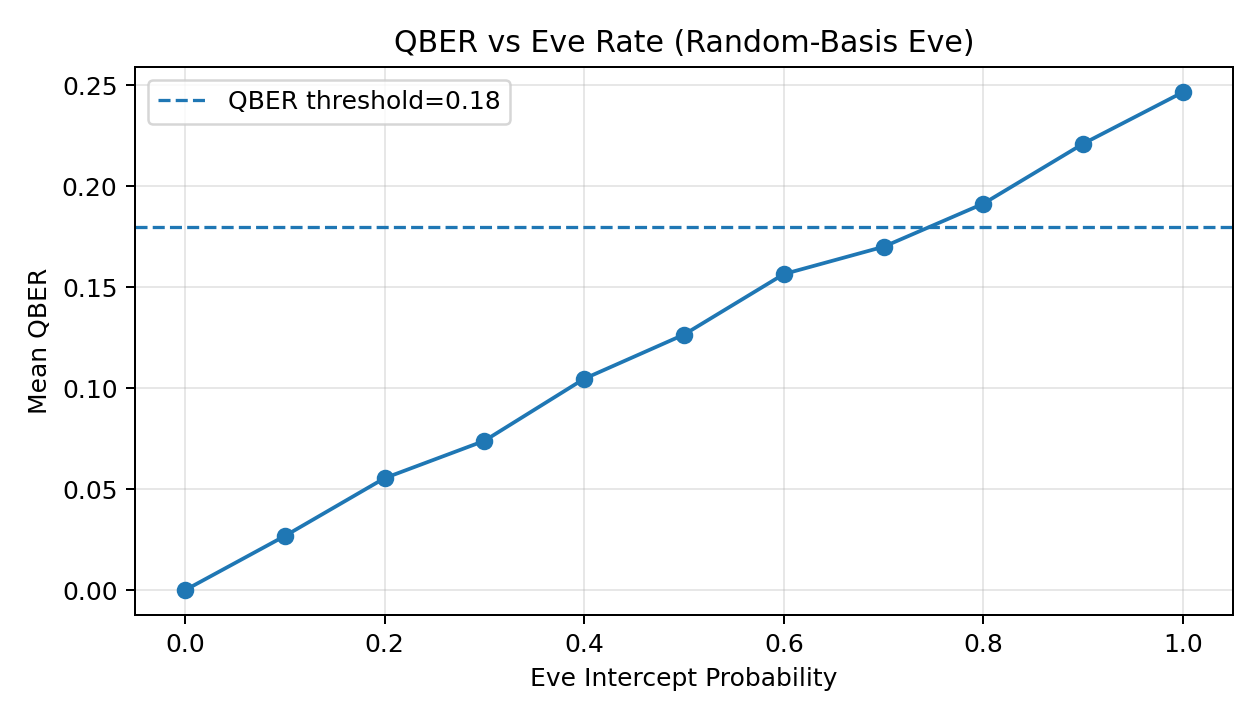
\includegraphics[width=0.85\linewidth]{figures/qber_vs_eve_rate_random.png}
  \caption{Mean QBER versus Eve interception rate in random-basis mode. Dashed line denotes acceptance threshold.}
\end{figure}

\begin{figure}[H]
  \centering
  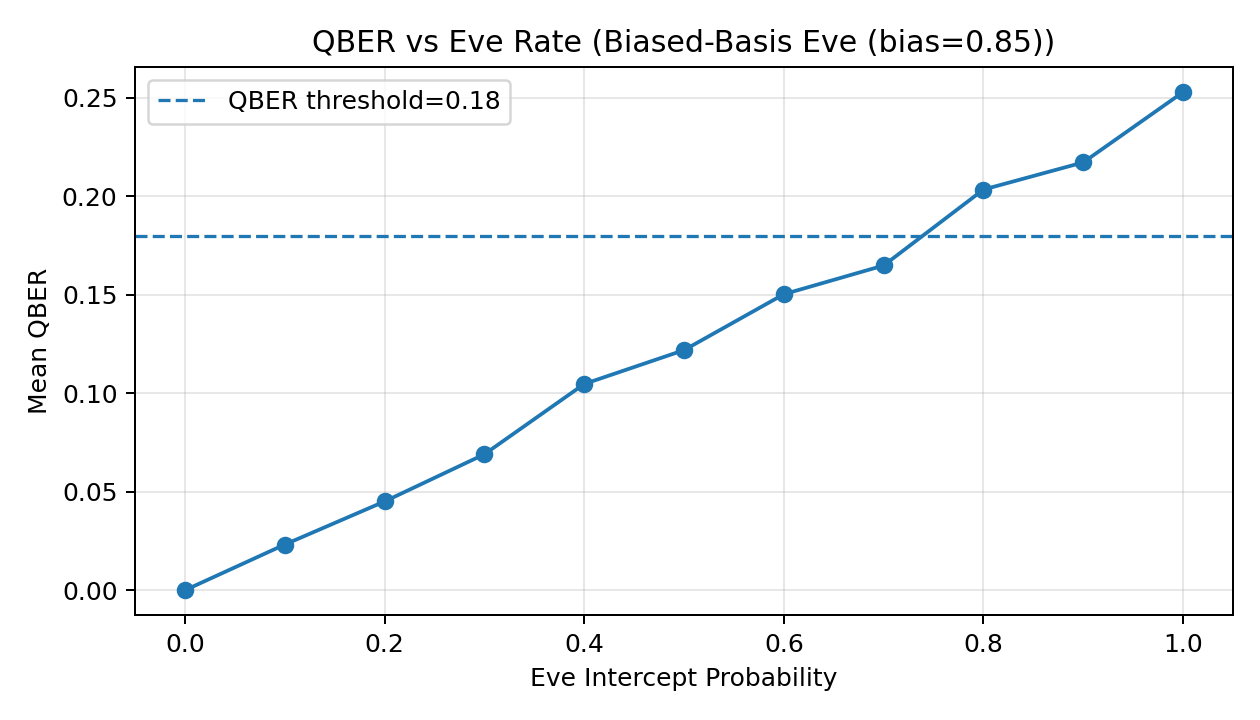
\includegraphics[width=0.85\linewidth]{figures/qber_vs_eve_rate_biased.png}
  \caption{Mean QBER versus Eve interception rate in biased mode ($p_X=0.85$).}
\end{figure}

\begin{figure}[H]
  \centering
  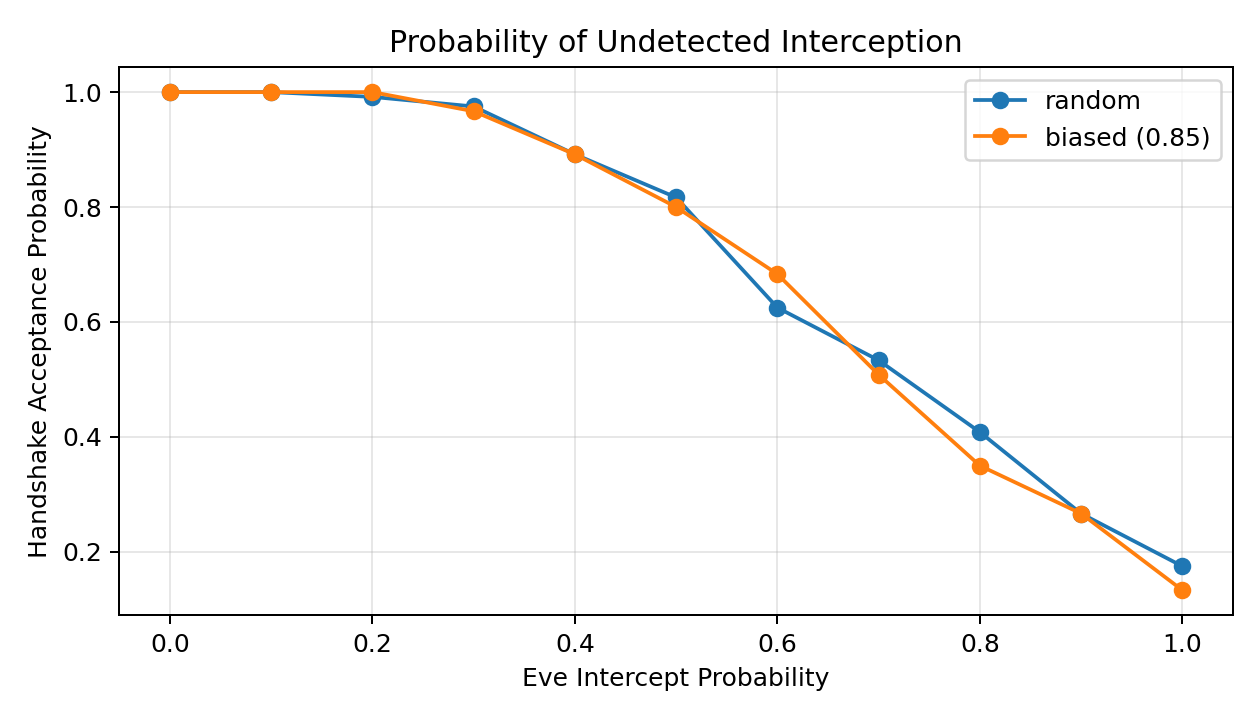
\includegraphics[width=0.85\linewidth]{figures/acceptance_vs_eve_rate.png}
  \caption{Handshake acceptance probability under increasing interception pressure.}
\end{figure}

\begin{figure}[H]
  \centering
  \begin{subfigure}{0.49\linewidth}
    \centering
    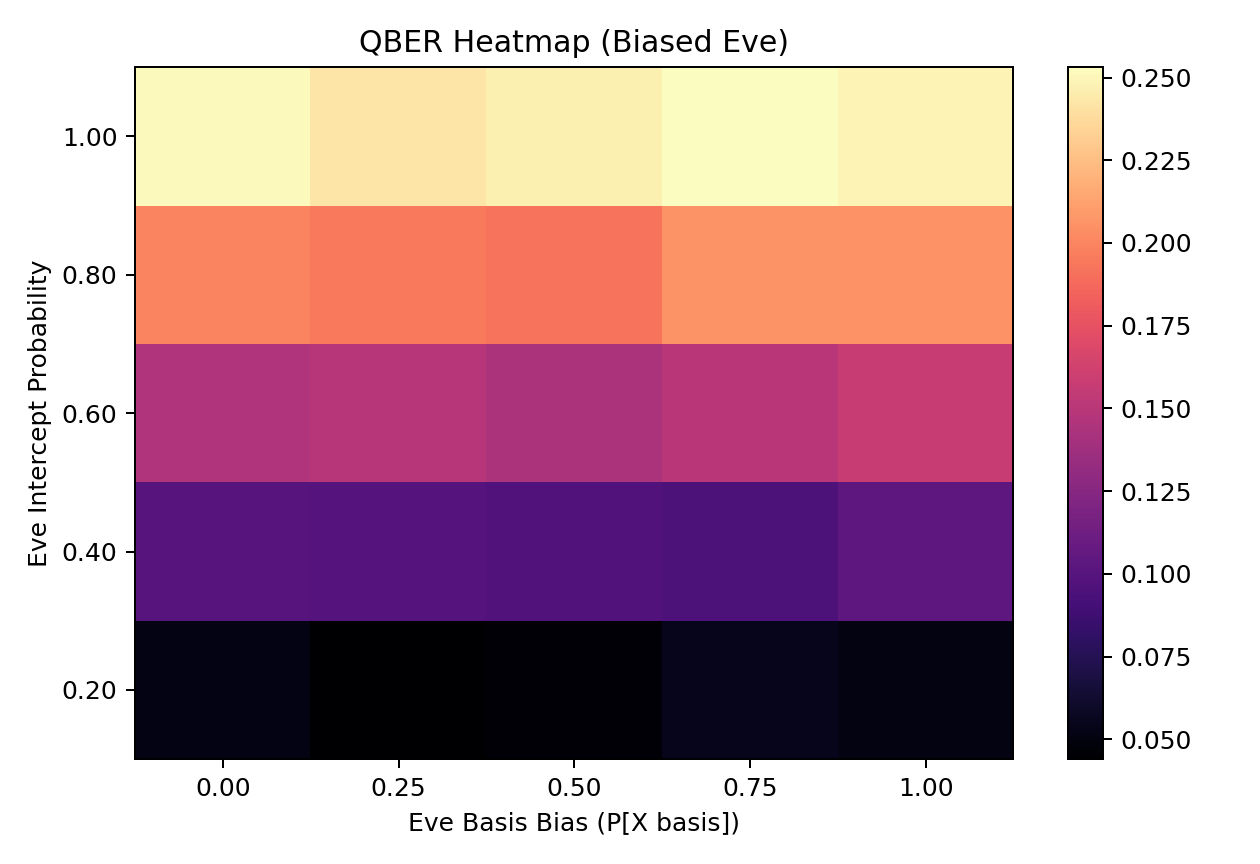
\includegraphics[width=\linewidth]{figures/heatmap_qber_bias_vs_rate.png}
    \caption{QBER surface}
  \end{subfigure}
  \hfill
  \begin{subfigure}{0.49\linewidth}
    \centering
    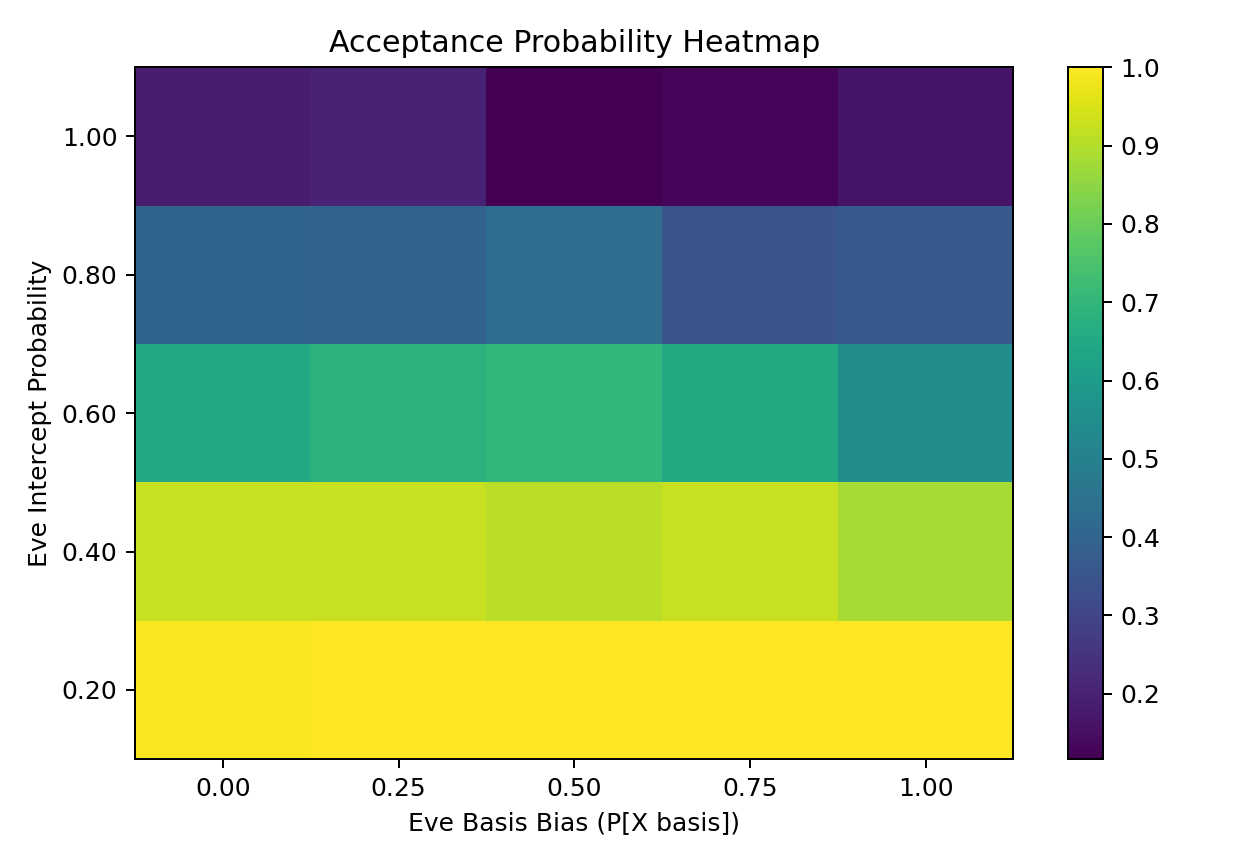
\includegraphics[width=\linewidth]{figures/heatmap_acceptance_bias_vs_rate.png}
    \caption{Acceptance surface}
  \end{subfigure}
  \caption{Sensitivity to Eve intercept rate and basis bias.}
\end{figure}

\subsection{Interpretation}
Empirical trends align with BB84 expectations:
\begin{itemize}[leftmargin=1.5em]
  \item QBER increases monotonically with higher interception probability.
  \item As QBER rises beyond threshold, session acceptance probability collapses.
  \item Biased-basis Eve strategies alter disturbance patterns, but sustained interception remains detectable.
\end{itemize}

From an attacker's perspective, remaining undetected requires keeping effective disturbance low. This implies a trade-off: stronger observation yields more information but significantly higher abort risk.

\section{Security Discussion}
\subsection{Strengths}
\begin{itemize}[leftmargin=1.5em]
  \item Disturbance-detection mechanism inherited from BB84 logic.
  \item Authenticated encryption with replay checks protects application traffic.
  \item Encrypted post-handshake authentication prevents plaintext credential leakage.
  \item Password hardening: PBKDF2 verifier, throttling, and lockout policy.
  \item Structured forensic logs for QKD reports, Eve activity, sessions, and commands.
  \item Persistent sessions reduce repeated handshakes and enable realistic remote operation workflows.
\end{itemize}

\subsection{Limitations}
\begin{itemize}[leftmargin=1.5em]
  \item QKD channel is simulated; no physical quantum hardware model.
  \item Endpoint trust and host-key pinning are out of scope.
  \item Side-channel and implementation-level leakage are not modeled.
  \item Current lockout identity is IP-based and may need refinement behind NAT/proxy topologies.
\end{itemize}

\subsection{Why Interception Becomes Hard}
In this prototype, \emph{hard to intercept} means difficult to extract large signal information while maintaining low detectability. As Eve increases intercept fraction, the observed QBER trend drives handshake rejections, sharply reducing successful covert sessions.

\section{Reproducibility Guide}
\subsection{Generate Figures}
From repository root:
\begin{verbatim}
.\.venv\Scripts\python scripts\generate_qkd_figures.py --trials 160
\end{verbatim}

\subsection{Build PDF}
If a LaTeX distribution is installed:
\begin{verbatim}
cd report
pdflatex qsh_research_report.tex
pdflatex qsh_research_report.tex
\end{verbatim}

\section{Conclusion and Future Work}
QSH demonstrates a complete research-grade pipeline: BB84-inspired key establishment, classical cryptographic channel transition, encrypted credential validation, and practical remote operations over persistent sessions. The implemented Eve scenarios and generated plots provide quantitative evidence of the expected BB84 disturbance-detection dynamics.

Immediate next steps include:
\begin{itemize}[leftmargin=1.5em]
  \item integrating richer channel noise and detector error models,
  \item extending authentication to asymmetric host/client credentials,
  \item adding integrity-protected audit shipping and anomaly scoring over logs,
  \item studying long-session rekeying strategies under dynamic QBER estimates.
\end{itemize}

\begin{thebibliography}{99}
\bibitem{bb84}
C. H. Bennett and G. Brassard, ``Quantum cryptography: Public key distribution and coin tossing,'' \emph{Proceedings of IEEE International Conference on Computers, Systems and Signal Processing}, 1984.

\bibitem{qiskit}
H. Abraham et al., ``Qiskit: An Open-source Framework for Quantum Computing,'' 2019. \url{https://qiskit.org/}

\bibitem{hkdf}
H. Krawczyk and P. Eronen, ``HMAC-based Extract-and-Expand Key Derivation Function (HKDF),'' RFC 5869, 2010.

\bibitem{gcm}
D. McGrew and J. Viega, ``The Galois/Counter Mode of Operation (GCM),'' NIST submission, 2004.

\bibitem{ssh}
T. Ylonen and C. Lonvick, ``The Secure Shell (SSH) Protocol Architecture,'' RFC 4251, 2006.
\end{thebibliography}

\end{document}
